% !TeX spellcheck = en_US
%\setcounter{chapter}{6} % set chapter counter so we begin at chapter 5
%\chapter{Laboration: PI/PID control of The Classroom Exo}


\section{Lab Introduction}

\begin{tcolorbox}[colback=blue!5!white,colframe=blue!75!black,title=Summary]
	In this chapter you will find the necessary documentation to setup your Classroom Exo, and try out the EMG options. We have prepared some Lab exercises, to help you learn more about surface Electromyography and control.
\end{tcolorbox}
\vspace{0.5cm}
 
An exoskeleton is a wearable mechanical structure that enhances or restores the physical abilities of the wearer by providing external support or amplification of movements \cite{AlTashi2024}. As the field of robotics grows leaps and bounds with every passing day as the world of STEM aims to integrate technology with humans to aid and support or enhance activities of daily living. Education leveraging these technologies has however been lacking. 
This lab is intended for use at a university level and is a derivative of a project aimed at converting an open-source exoskeleton into educational material \cite{AlTashi2024}. The Classroom Exo, the product that we will be using through the course of this lab, is a student-friendly optimized version of the EduExo Pro - An Advanced Robotic Exoskeleton Kit developed by Auxivo AG. 

\subsection{Risk section}
The Classroom Exo is not categorized as a medical device. Instead, its primary focus is educational. It is designed to provide hands-on experience with various control systems. There are some risks associated with the use of the Classroom Exo. Listed below are the potential risks, what has been done to prevent them, and the possible causes of these risks.
\begin{itemize}[]
	\item \textbf{Muscle fatigue:} Muscle fatigue can occur during prolonged use, as the Classroom Exo is somewhat heavy. To minimize this risk, an ergonomic design and proper usage guidelines have been implemented.
	\item \textbf{Skin irritation:} Some users have experienced skin irritation from reacting to surface electrodes. Although it is uncommon, skin-friendly materials are used to minimize this risk. Irritation typically occurs after prolonged contact with the EMG sensors.
	\item \textbf{Injury risk:} The risk of injury is very low, but it still exists. The primary cause is misalignment between the Classroom Exo's mechanical joints and the user's shoulder and elbow joints. This risk has been minimized through proper calibration, an emergency stop feature, and clear instructions for how to put on the Classroom Exo.
\end{itemize}
	
\subsection{Learning objectives}
The goal of this section is to explore how EMG signals are generated from muscle activity and can be used to control a system. You will be introduced to basic anatomy and physiology to assist with electrode placement and reflect on the challenges of using biological signals, including signal strength, interference, reference signals, signal propagation, and processing. 

\begin{itemize}[]
	\item Set up the EMG measurement system to control exoskeleton movement.
	\item Troubleshoot and resolve common EMG-related signal setup issues and evaluate how different factors affect the measured signal. 
	\item Reflect on applications of EMG-controlled systems in terms of use cases and patient safety. 
	
\end{itemize}
	
\subsection{Prerequisite knowledge}
The prerequisite knowledge for this section is basic engineering principles such as signal propagation, disturbance signals, and signal processing. Knowledge of basic muscle physiology yields an optimal experience in this lab. Our recommendation would be to introduce this section in the first year of a biomedical engineering programme; however, this could be introduced later or earlier (with some preparations from the teacher) and still be beneficial for the students.  

\subsection{Materials and methods}
For this lab, you will need a Bluetooth-enabled computer and MATLAB 2023b (although newer versions should also work). We will be interfacing with the exoskeletons using the “Updated BT-GUI” MATLAB application. Additionally, you will need one exoskeleton and a screwdriver to adjust the arm length of the exoskeleton to fit the anatomy of the student who will be wearing the exoskeleton. For the EMG control, you will need three electrodes and one/two Myoware sensors (depending on the number of channels used). 

\subsection{To do at home before the lab}
To make the most of the limited time you will have with the exoskeletons, you must come to the lab session well-prepared. Unforeseen issues or complications with the setup of the exoskeletons may arise, so proper preparation will ensure you have as much hands-on time as possible with the exoskeleton. Therefore before the lab asks you to:  
\begin{enumerate}[]
	\item Download MATLAB 2023b.
	\item Download the “Updated BT-GUI\_10-24”  folder from the GitHub link: \url{https://github.com/fabianjust/classroom-exo}
	\item Download and install the following MATLAB packages: 
	\begin{itemize}[]
		\item Control System Toolbox (version 23.2)
		\item Instrument Control Toolbox (version 23.2)
		\item Robotics System Toolbox (version 23.2)
		\item Sensor Fusion and Tracking Toolbox (version 23.2)
		\item Signal Processing Toolbox (version 23.2)
		\item Symbolic Math Toolbox (version 23.2)
	\end{itemize}
	\item Read the lab PM thoroughly.
\end{enumerate}


\newpage
	
\section{Introduction to the Exoskeleton}
Exoskeletons are increasingly being incorporated into rehabilitative settings, such as walking assists for people who have undergone spinal cord injuries, strokes, etc., in physiotherapy, and occupational therapy \cite{Hill2017}. Although aimed to be used in educational settings only, the Classroom Exo is an exoskeleton connected to the upper part of the body, over the shoulder, and the upper and lower arm, with a spring support to help lift the arm \autoref{fig:fig02}. Programmed on Arduino, it has three control systems - proportional–integral–-derivative controller (PID Controller), Electromyography signals from the muscles, and a force sensor on the wrist, the software of which is accessible as open-source, with a classroom-friendly graphical interface implemented on MATLAB. 

\begin{figure}[H]
	\centering
	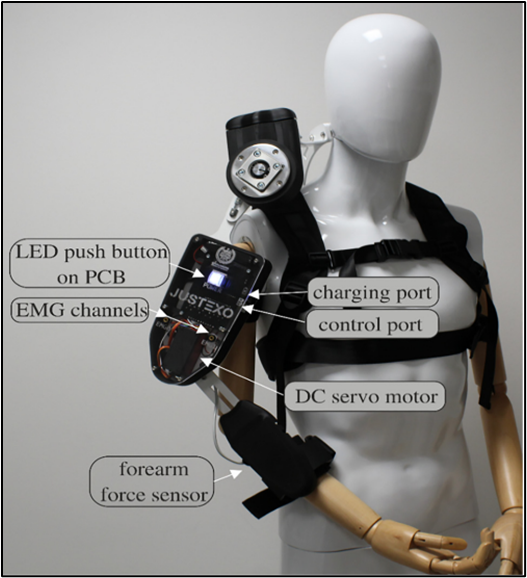
\includegraphics[width=0.7\linewidth]{img/fig_02}
	\caption{The Classroom Exo and its adaptations from EduExo Pro }
	\label{fig:fig02}
\end{figure}

\subsection{Setting up the Classroom Exo}
While putting on the exoskeleton it is helpful if one person holds it up and another tightens the straps.
\begin{enumerate}[]
	\item Put on the vest and fasten the buckles. 
	\item Make sure that the shoulder part of the exoskeleton is aligned with your shoulder, which can be seen in \autoref{fig:fig03}. And then tighten the chest and waist straps.
\end{enumerate}

\begin{figure}[H]
	\centering
	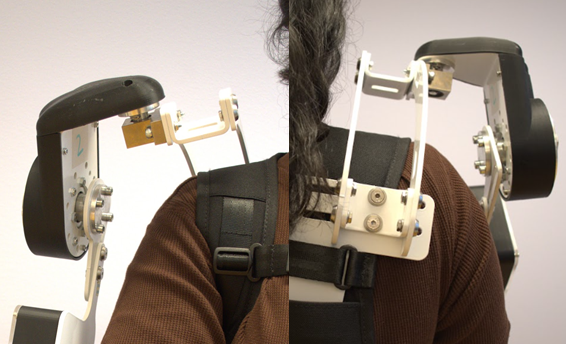
\includegraphics[width=0.4\linewidth]{img/fig_03}
	\caption{Shoulder joint aligned (left) and misaligned (right).}
	\label{fig:fig03}
\end{figure}

\begin{enumerate}[]
	\setcounter{enumi}{2}
	\item Tighten the straps around the elbow and the wrist and check alignment with the elbow joint according to \autoref{fig:fig04}. 
\end{enumerate}

\begin{figure}[H]
	\centering
	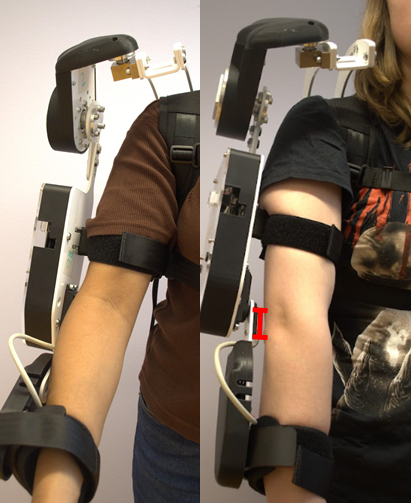
\includegraphics[width=0.4\linewidth]{img/fig_04}
	\caption{Correct alignment of elbow joint (left) and incorrect alignment (right), misalignment marked in red.}
	\label{fig:fig04}
\end{figure}

\begin{enumerate}[]
	\setcounter{enumi}{3}
	\item If the Classroom Exo has the correct joint alignment as seen in figure 4 and 3, proceed to section 2.1.2. If not, proceed with section 2.1.1 “Adjusting the exoskeleton”.
\end{enumerate}

\subsubsection{Adjusting the exoskeleton}
To be able to adjust the arm length of the Classroom Exo, a 2.5 and 3.0 Allen Key is needed.

\begin{enumerate}[]
	\item Under the shoulder joint on the back of the exoskeleton you can find two bolts for which the 3.0 Allen Key fits, the bolts are marked in \autoref{fig:fig05}. Loosen these, align shoulder joints according to \autoref{fig:fig03} and tighten the bolts. 
\end{enumerate}



\begin{figure}[H]
	\centering
	\begin{center}
		\begin{tikzpicture}
			\node(a){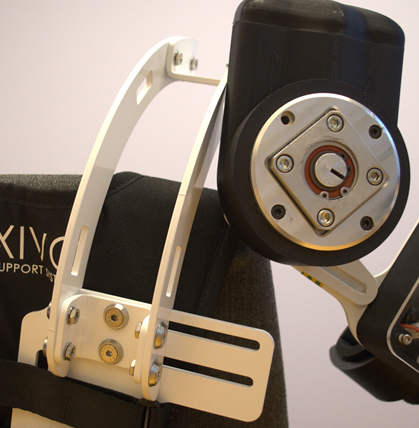
\includegraphics[width=0.4\linewidth]{img/fig_05}};
			\node at(a.center)[draw, red,line width=3pt,circle, minimum width=45pt, minimum height=45pt,rotate=-40,yshift=-65pt]{};
		\end{tikzpicture}   
	\end{center}
	\caption{Bolts for adjusting shoulder breadth in red.}
	\label{fig:fig05}
\end{figure}



\begin{enumerate}[]
	\setcounter{enumi}{1}
	\item To align the elbow, loosen the bolts on the inside of the shoulder joint illustrated in \autoref{fig:fig06}. Use the 3.0 Allen key to do this. Slide the arm such that the elbow joint of the exoskeleton and the user is aligned such as in \autoref{fig:fig04}. Tighten the bolts.
\end{enumerate}

\begin{figure}[H]
	\centering
	\begin{center}
		\begin{tikzpicture}
			\node(a){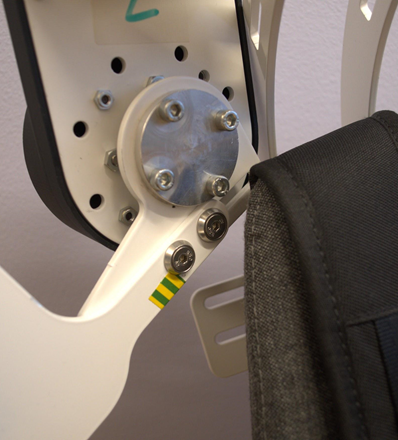
\includegraphics[width=0.4\linewidth]{img/fig_06}};
			\node at(a.center)[draw, red,line width=3pt,circle, minimum width=45pt, minimum height=45pt,rotate=0,yshift=-7pt, xshift=-1pt]{};
		\end{tikzpicture}   
	\end{center}
	\caption{Bolts to adjust upper arm length for elbow alignment marked in red.}
	\label{fig:fig06}
\end{figure}



\begin{enumerate}[]
	\setcounter{enumi}{2}
	\item To adjust the position of the wrist cuff, loosen the bolt on the lower part on the arm of the exoskeleton marked in \autoref{fig:fig07}, using the 2.5 Allen key. Adjust length and tighten the bolts.
\end{enumerate} 

\begin{figure}[H]
	\centering
	\begin{center}
		\begin{tikzpicture}
			\node(a){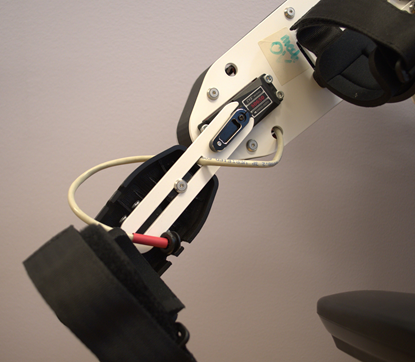
\includegraphics[width=0.4\linewidth]{img/fig_07}};
			\node at(a.center)[draw, red,line width=3pt,circle, minimum width=15pt, minimum height=15pt,rotate=0,xshift=-12pt, yshift=-2pt]{};
		\end{tikzpicture}   
	\end{center}
	\caption{Bolts to adjust lower arm length for positioning of wrist cuff marked in red.}
	\label{fig:fig07}
\end{figure}
\subsubsection{Connecting to the device and starting the GUI}
\begin{enumerate}[]
	\item Turn on the exoskeleton by pushing the “LED push button on PCB” as seen in \autoref{fig:fig08}. It  should blink blue indicating that it is searching for a Bluetooth device.
	\item When you are connecting to the exoskeleton for the first time, go to your computer's Bluetooth settings and add a Bluetooth device. When pairing, the name of your device will be XX\_CLASSROOM\_EDU\_EXO\_PRO where the XX is a number between 01 to 08 depending on which exoskeleton you have.
\end{enumerate}

\begin{figure}[H]
	\centering
	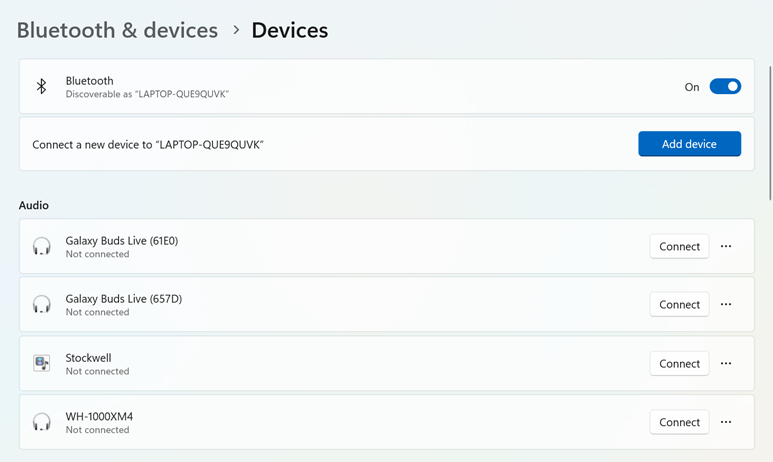
\includegraphics[width=0.7\linewidth]{img/fig_08}
	\caption{Pairing to a Bluetooth device for the first time.}
	\label{fig:fig08}
\end{figure}
\begin{enumerate}[]
	\setcounter{enumi}{2}
	\item In your computer's display settings set the screen size to 100\%.
\end{enumerate}
\begin{figure}[H]
	\centering
	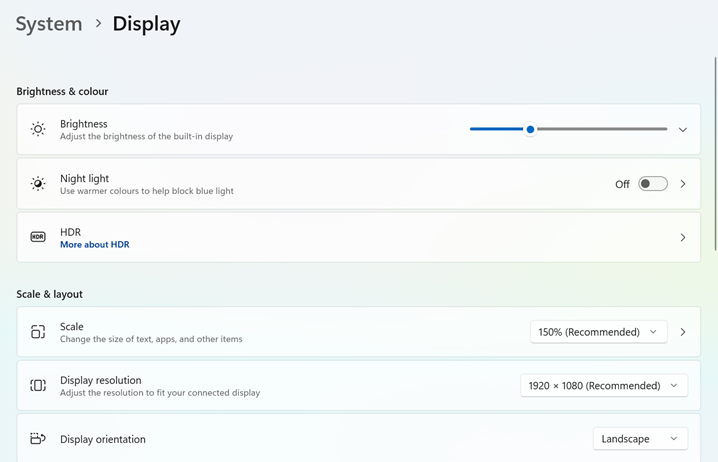
\includegraphics[width=0.7\linewidth]{img/fig_09}
	\caption{Changing screen sizing.}
	\label{fig:fig09}
\end{figure}

\begin{enumerate}[]
	\setcounter{enumi}{3}
	\item Open MATLAB, locate the BT\_GUI file and double click on it. Or locate the file in your file explorer and select open with MATLAB. If you open the file in MATLAB’s app designer, click run.
	\item When the GUI is opened, choose the correct Bluetooth device, and click connect. 
\end{enumerate}

\begin{figure}[H]
	\centering
	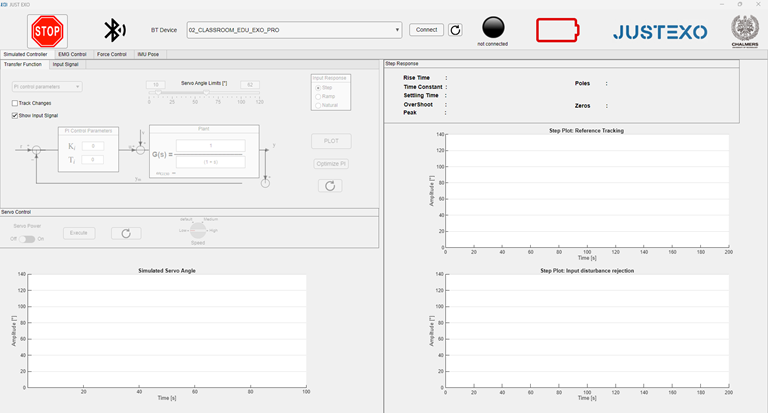
\includegraphics[width=0.7\linewidth]{img/fig_10}
	\caption{Connecting to the Bluetooth device.}
	\label{fig:fig10}
\end{figure}

The power button on the exoskeleton and the indicator in the GUI should change color to either green, yellow or red depending on the battery level.


\newpage
\section{EMG controller}
\subsection{Introduction}
The technique to measure motor control - the electrical activity from the muscles in the human body is called Electromyography (EMG). Every time our muscles contract and expand, a difference in electrical potential can be observed, which can be measured using surface electrodes (surface or sEMG). The Classroom Exo uses a popular and well-accredited sEMG sensor called the Myoware sensor as shown in \autoref{fig:fig10}, which is easy to use and interface with the microcontroller and comes with a built-in filtering system that transforms raw EMG signal into usable readings (enveloped signal) \cite{AlTashi2024}.

\begin{figure}
	\centering
	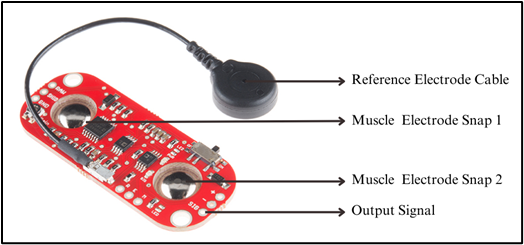
\includegraphics[width=0.7\linewidth]{img/fig_11}
	\caption{Sensor Layout - MyoWareTM Muscle Sensor (AT-04-001) \cite{Myoware}.}
	\label{fig:fig11}
\end{figure}
 

The Classroom Exo implements a threshold-based control system using two MyoWare muscle sensors integrated with the PCB. The current system can accommodate two sEMG sensors connected to the PCB via insulated AUX cables (a 2-channel EMG control system). Each muscle sensor has two electrodes and a reference electrode \cite{AlTashi2024}. The sensor should be placed on the muscle intended to control the exoskeleton (here, the biceps/triceps brachii), and the reference electrode (preferably a bony part on your elbow). The muscle electrical activity can be broken down as follows: when you flex your arm, the biceps contract, and when you extend your arm, your triceps contract. 

\begin{figure}
	\centering
	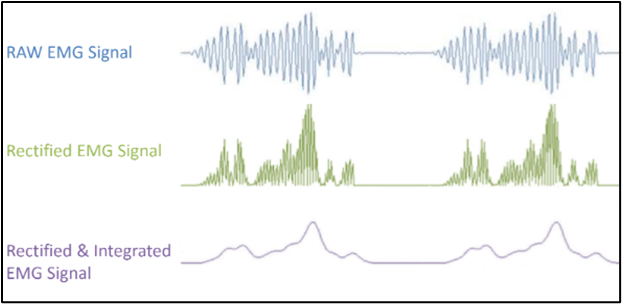
\includegraphics[width=0.7\linewidth]{img/fig_12}
	\caption{Representation of the EMG signal before and after passing it through the sensor [4].}
	\label{fig:fig12}
\end{figure}

The electrode placement as shown in \autoref{fig:fig12}, is pivotal to getting steady and strong signals. These arm movements in turn control the servo movements in the hardware. When the amplitude of the EMG signal exceeds a set threshold, the servo motor contracts the arm of the exoskeleton. When the amplitude of the EMG signal goes under a set lower threshold, the servo motor of the exo moves in the other direction thus extending the arm. We can monitor the amplitude of the enveloped signals in real-time graphs on the MATLAB GUI and manually set the threshold values. 

\begin{figure}
	\centering
	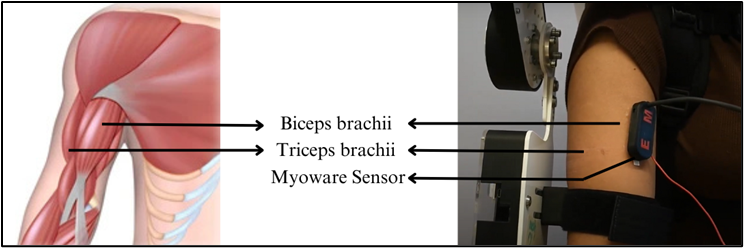
\includegraphics[width=0.7\linewidth]{img/fig_13}
	\caption{Electrode Placement and Muscle Anatomy \cite{Muscles}. }
	\label{fig:fig13}
\end{figure}


\newpage
\subsection{EMG setup}
The exoskeleton should be put on before attaching the sEMG sensor. 
1.	Take out the sEMG sensors and three surface electrodes from the plastic bag.
2.	Attach the surface electrodes (before removing them from the plastic) to the EMG sensors \autoref{fig:fig14}. 


\begin{figure}[H]
	\centering
	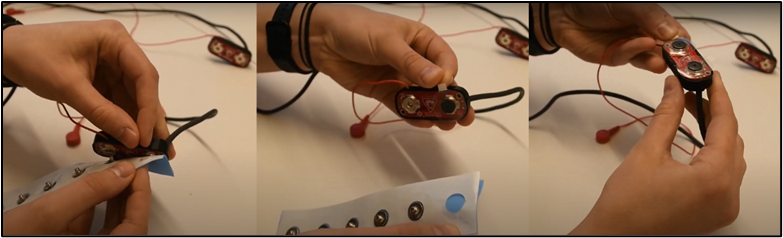
\includegraphics[width=0.7\linewidth]{img/fig_14}
	\caption{Attaching the surface electrodes to the sensor.}
	\label{fig:fig14}
\end{figure}


3.	Attach the EMG sensor to the bicep and plug the AUX cable into the Classroom Exo to channel zero or one \autoref{fig:fig15}.  

\begin{figure}[H]
	\centering
	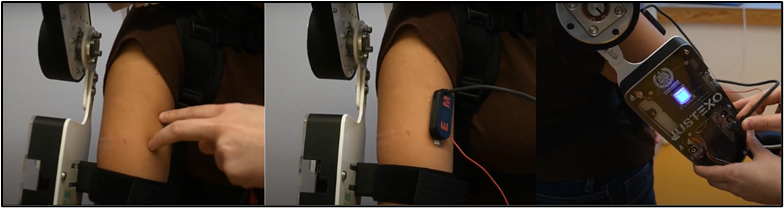
\includegraphics[width=0.7\linewidth]{img/fig_15}
	\caption{Placing the EMG sensor on the bicep and plugging in the AUX cable to the preferred channel.}
	\label{fig:fig15}
\end{figure}

4.	Attach the reference cable (red one) on the bony part of the elbow with a surface electrode on it \autoref{fig:fig16}.  

\begin{figure}[H]
	\centering
	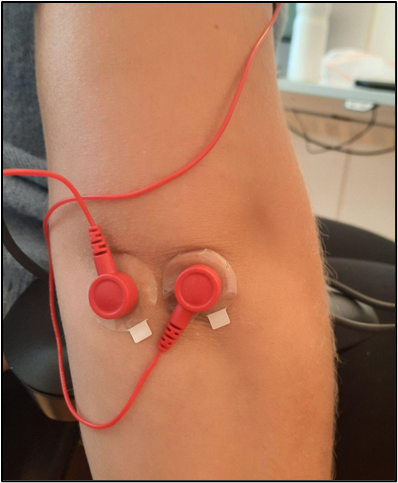
\includegraphics[width=0.4\linewidth]{img/fig_16}
	\caption{Placing the reference cable on the elbow.}
	\label{fig:fig16}
\end{figure}

5.	As shown in \autoref{fig:fig17}, choose the tab “EMG control” in the GUI. 

\begin{figure}[H]
	\centering
	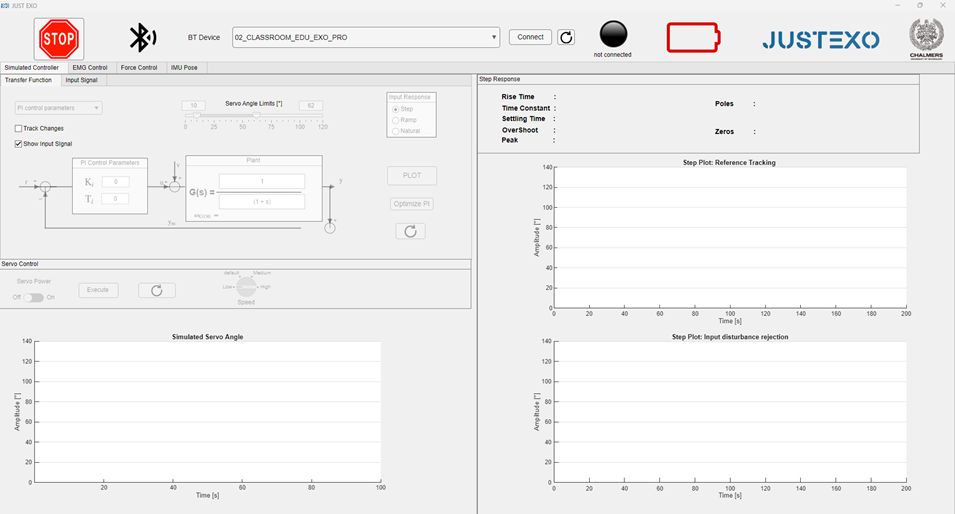
\includegraphics[width=0.7\linewidth]{img/fig_17}
	\caption{Choosing the EMG control tab.}
	\label{fig:fig17}
\end{figure}


6.	In the drop-down menu, choose the EMG channel selected when you plugged in the EMG sensor to the Classroom Exo.  
\begin{figure}[H]
	\centering
	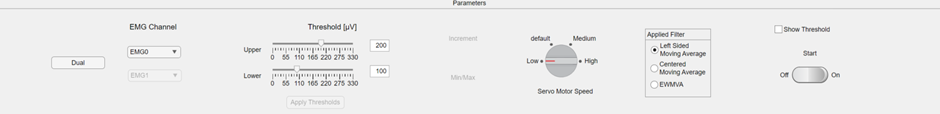
\includegraphics[width=1\linewidth]{img/fig_18}
	\caption{Choosing the EMG channel.}
	\label{fig:fig18}
\end{figure}




7.	Before you click on start, you can control if the EMG sensor is on by checking if the little lights in the EMG sensor are blinking. It should blink green if it has power, and red if it detects muscle activity as observed in \autoref{fig:fig19}. 

\begin{figure}[H]
	\centering
	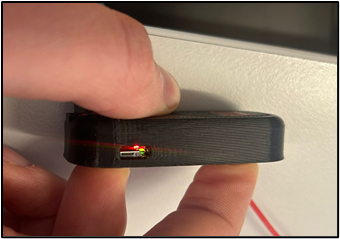
\includegraphics[width=0.4\linewidth]{img/fig_19}
	\caption{Lighhts corresponding to power and muscle potential on the eMG sensor.}
	\label{fig:fig19}
\end{figure}

8.	Click on the start button. 
9.	If you can see the curve changing when flexing your muscle, but the Classroom Exo does not move, then you can stop running and adjust the threshold. This is done by dragging the mark along the bar with numbers below the Threshold title at the bottom of the GUI as in \autoref{fig:fig20}. You can change both the upper and lower thresholds. 


\begin{figure}[H]
	\centering
	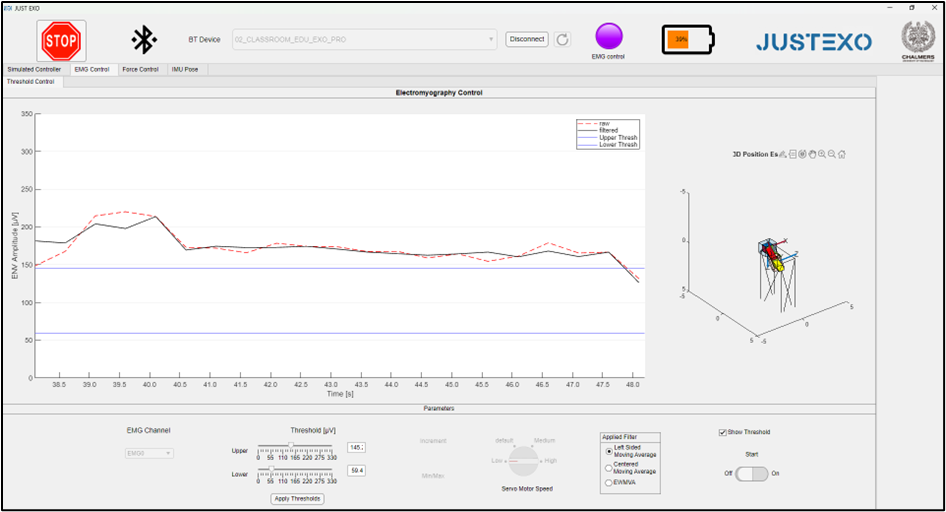
\includegraphics[width=0.7\linewidth]{img/fig_20}
	\caption{Adjusting the threshold in the GUI.}
	\label{fig:fig20}
\end{figure}

\newpage
\section{Exercises}
This section outlines a series of exercises to be completed during the allotted lab time. These exercises are designed to deepen your understanding of how EMG control can be applied in combination with the Classroom Exo. 

\subsection{Tasks and questions}

\begin{enumerate}[]
	\item Flex your bicep, if the EMG signal exceeds the upper threshold, you should see the exoskeleton move.  
	\begin{enumerate}[]
		\item Disconnect the reference electrode. Do you notice any difference from before, why? 
		\item Change the position of the reference electrode to: 
		\begin{enumerate}[]
			\item the same muscle as the body of the sensor (the bicep)
			\item a muscle in the opposite arm. Do you notice a difference, why? 
			\textbf{Reposition the reference electrode to the bony part after this exercise.}
		\end{enumerate}
	\end{enumerate}
\end{enumerate}
 
\begin{enumerate}[]
	\item Flex your bicep, if the EMG signal exceeds the upper threshold, you should see the exoskeleton move.  
	\begin{enumerate}[]
		\item Try different sensor positions:  
		\begin{enumerate}[]
			\item Rotate the sensor 180 degrees to change its orientation. 
			Do you see any alterations in the output signal? Why/why not? 
			\item Move the electrodes farther away from the central part of the target muscle. 
			How does the signal strength/quality change? 
		\end{enumerate}
	\end{enumerate}
\end{enumerate}
	
\begin{enumerate}[]
	\item What are the default threshold limits?  
	\begin{enumerate}[]
			\item Lower both thresholds, click “apply thresholds” and restart the start button. 
			\item What does controlling the exoskeleton feel like now? 
			\item What would the applications be for lowering the limits? 
			\textbf{Revert to the default threshold limits after the exercise.} 
	\end{enumerate}
\end{enumerate}

\begin{enumerate}[]
	\item 	When the sensor is on, try different movements: 
	\begin{enumerate}[]
		\item Move your arm around instead of extending or flexing it. What changes do you observe with the signal? 
		\item Walk around while still wearing the exoskeleton. What changes do you observe with the signal during these movements? 
		\item How can we describe what you observe in terms of disturbance signals (external factors like the environment, body movement, etc.) and sensitivity of the sensor? 	
	\end{enumerate}
\end{enumerate}

	 
\begin{enumerate}[]
	\item Try different muscles:
	\begin{enumerate}[]
		\item Switch to a different muscle (this might be easier if you remove the exo from your body). Try using a larger or smaller muscle, for example, Gastrocnemius (the calf), etc. 
		\begin{figure}
			\centering
			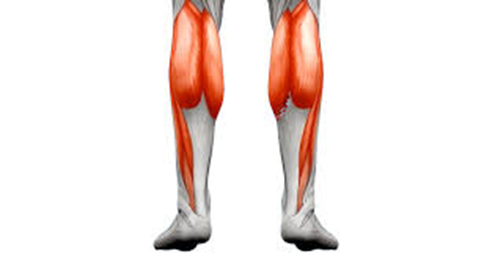
\includegraphics[width=0.7\linewidth]{img/fig_21}
			\caption{Try placing the sensor on the calf muscle instead of the Biceps \cite{Walden2022}.}
			\label{fig:fig21}
		\end{figure}
		\item Observe and note how high the muscle activity is in each of your target muscles. 
		\item What would be the application of controlling an exoskeleton with another muscle? For example, what would be a real-life application to use the calf muscle to control elbow flexion in an upper body exoskeleton? 
	\end{enumerate}
\end{enumerate}
	

\begin{enumerate}[]
	\item Dual Channel: Connect one of the EMG sensors to the Biceps (say EMG0), and the other to the Triceps (say EMG1). Click on the dual button to activate both channels. Note that each channel now corresponds to one of the thresholds and the servo changes direction if it crosses the upper or lower thresholds. 
\end{enumerate}


\begin{figure}
	\centering
	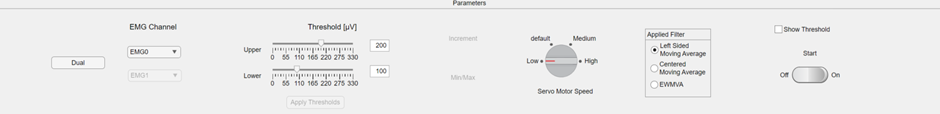
\includegraphics[width=1\linewidth]{img/fig_22}
	\caption{Choosing the dual channel mode. }
	\label{fig:fig22}
\end{figure}


Flex your bicep. If  EMG0 exceeds the upper threshold, you should see the exoskeleton move, and as you relax, and EMG1 exceeds the lower threshold you should see the exoskeleton extend as well. 
\begin{enumerate}[]
	\item How are the mono and dual modes different from each other? Do you see anyone having an advantage over another? 
	\item How can these two modes be deployed in real-life applications of the exoskeleton and more? 
\end{enumerate}
 
\subsection{Discussion}
For the best learning experience, feel free to discuss the results your group obtained from each step between groups to gain understanding and new perspectives.

\begin{enumerate}[]
	\item What differed between your answers and the answers of other groups?
	\item Why did your answers or conclusions differ?
	\item Did your discussions between groups lead to new insights or ideas? If so, what were they?
\end{enumerate}

\section{Typical Errors and Troubleshooting}
In this section, we present typical errors and issues encountered during testing of the Classroom Exo.


\begin{enumerate}[]
	\item If the EMG does not start (green lights start blinking) try changing the EMG sensor or channel. You could also try wiping the area where the electrodes are placed with a wet wipe before putting the sensor on the skin. 
	\item If the thresholds are not showing or the signal is not showing after changing the thresholds, then click “apply thresholds” and turn the start button off and then on again. Wait for the signal to appear. 
	
\end{enumerate}	
	 
\begin{figure}[H]
	\centering
	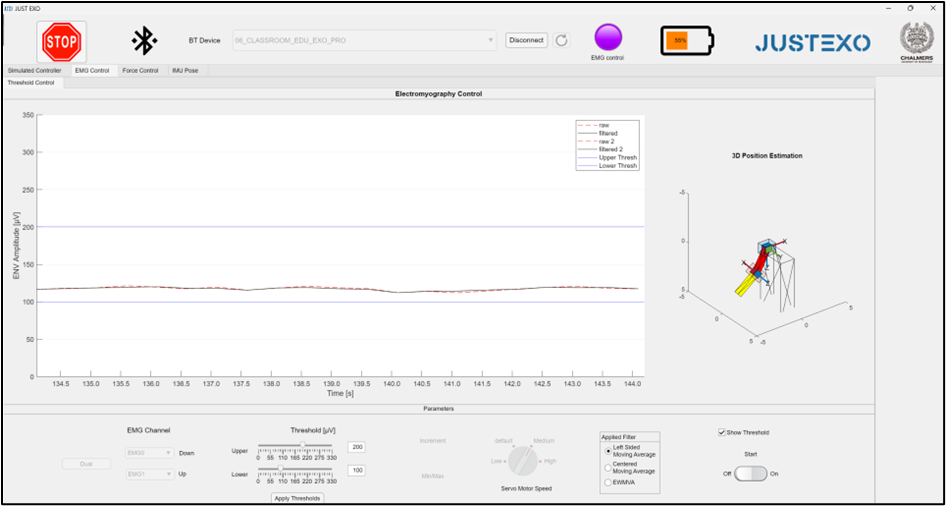
\includegraphics[width=0.7\linewidth]{img/fig_23}
	\caption{Steady signal corresponding to having chosen the wrong EMG channel. }
	\label{fig:fig23}
\end{figure}

\begin{enumerate}[]
	\setcounter{enumi}{2}
	\item If nothing happens when you flex your muscle, and the signal does not change: 
	\begin{enumerate}[]
		\item Make sure the sensor is intact on the arm. 
		\item Check if the EMG is actually powered (the green light should be on), if it receives signals the red light should be blinking. 
		\item Check your connections with the AUX cable to the exo, and the sensor wires. A loose connection could be causing trouble. 
		\item Switch to a different sensor if the issue persists. 
	\end{enumerate}
	\item If you are having trouble with the EMG signal for example steady low/steady high signal, try checking the connection with the aux cable and the connection with the electrodes (push it in). 
	\item When the person who is wearing the electrode touches a computer at the same time as the GUI runs, the signal might be erratic and unsteady. 
	\item If you get a constant and steady signal, maybe you have chosen the wrong channel.
\end{enumerate}

\begin{tcolorbox}[colback=green!5!white,colframe=green!75!black,title=Hint]
	You can find a more comprehensive Troubleshooting documentation in the Manual on our GitHub!
\end{tcolorbox}
\vspace{0.5cm}


	




